%\title{LaTeX Portrait Poster Template}
%%%%%%%%%%%%%%%%%%%%%%%%%%%%%%%%%%%%%%%%%
% a0poster Portrait Poster
% LaTeX Template
% Version 1.0 (22/06/13)
%
% The a0poster class was created by:
% Gerlinde Kettl and Matthias Weiser (tex@kettl.de)
%
% This template has been downloaded from:
% http://www.LaTeXTemplates.com
%
% License:
% CC BY-NC-SA 3.0 (http://creativecommons.org/licenses/by-nc-sa/3.0/)
%
%%%%%%%%%%%%%%%%%%%%%%%%%%%%%%%%%%%%%%%%%

%----------------------------------------------------------------------------------------
%	PACKAGES AND OTHER DOCUMENT CONFIGURATIONS
%----------------------------------------------------------------------------------------

\documentclass[a0,portrait]{a0poster}
\usepackage{multicol} % This is so we can have multiple columns of text side-by-side
\columnsep=100pt % This is the amount of white space between the columns in the poster
\columnseprule=3pt % This is the thickness of the black line between the columns in the poster

\usepackage[svgnames]{xcolor} % Specify colors by their 'svgnames', for a full list of all colors available see here: http://www.latextemplates.com/svgnames-colors
\usepackage{tcolorbox}
\usepackage{tikz}
\usepackage{times} % Use the times font
%\usepackage{palatino} % Uncomment to use the Palatino font

\usepackage{graphicx} % Required for including images
\graphicspath{{figures/}} % Location of the graphics files
\usepackage{booktabs} % Top and bottom rules for table
\usepackage[font=small,labelfont=bf]{caption} % Required for specifying captions to tables and figures
\usepackage{amsfonts, amsmath, amsthm, amssymb} % For math fonts, symbols and environments
\usepackage{wrapfig} % Allows wrapping text around tables and figures

\begin{document}

%----------------------------------------------------------------------------------------
%	POSTER HEADER
%----------------------------------------------------------------------------------------

% The header is divided into two boxes:
% The first is 75% wide and houses the title, subtitle, names, university/organization and contact information
% The second is 25% wide and houses a logo for your university/organization or a photo of you
% The widths of these boxes can be easily edited to accommodate your content as you see fit

\begin{minipage}[b]{0.99\linewidth}
	\begin{center}
		\veryHuge \color{DarkRed} \textbf{On reverse-engineering natural computation} \color{Black}\\ % Title
		\Huge\textit{using reaction-diffusion approaches beyond linear stability}\\[2.4cm] % Subtitle
		\huge \textbf{Gregory Sz\'ep$^1$, Attila Csik\'asz-Nagy$^1$, Luca Cardelli$^2$}\\[0.5cm]
		\vspace{1cm}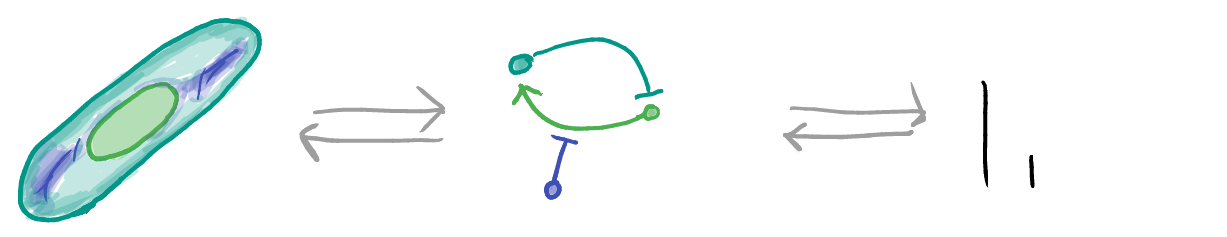
\includegraphics[width=70cm]{abstract}
	\end{center}
\end{minipage}

\addtobeamertemplate{}{}
{\begin{tikzpicture}[remember picture, overlay]
     \node [anchor=north west, inner sep=6cm]  at (-8,34)
     {
\includegraphics[height=7cm]{kcl}\huge $^2$};
  \end{tikzpicture}}

\addtobeamertemplate{}{}
{\begin{tikzpicture}[remember picture, overlay]
     \node [anchor=north east, inner sep=6cm]  at (83,34)
     {
\includegraphics[height=3cm]{mrc}\huge $^1$};
  \end{tikzpicture}}

	\addtobeamertemplate{}{}
	{\begin{tikzpicture}[remember picture, overlay]
	     \node [anchor=south west, inner sep=6cm]  at (-8,-88)
	     {
\includegraphics[height=7cm]{epsrc}};
	  \end{tikzpicture}}

%----------------------------------------------------------------------------------------

\begin{multicols}{3} % This is how many columns your poster will be broken into, a portrait poster is generally split into 2 columns

\section{Evolution of response behaviour}

Specific mappings have been explored between between algorithms, electrical
engineering circuits and chemical reaction networks \cite{}. Understanding function
of large biochemical networks from a computer science perspective guides experiments
in synthetic biology and in-vitro reconstructive approaches \cite{}.
\\
\begin{tcolorbox}[boxrule=2pt,arc=3.4pt,boxsep=2mm]
\begin{center}\color{DarkRed}
\textbf{How does one design the \textit{least complex} chemical
reaction network that obeys a given \textit{response function}?}
\end{center}
\end{tcolorbox}
\begin{center}
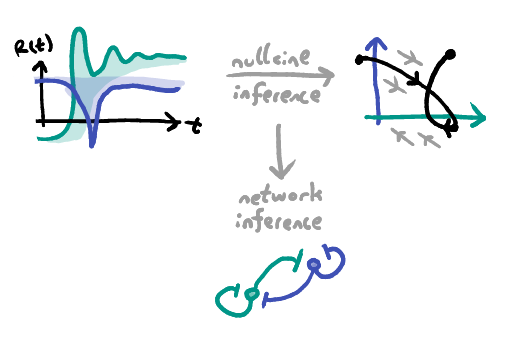
\includegraphics[width=1.0\linewidth]{inference}
\end{center}\noindent
The function of known biochemical networks such as the MAPK pathway,
circadian rhythms and cell-cycles can be understood in terms of simple
response functions; decomposition of large networks into switches and
clocks are proposed in literature.
\\\\
The networks found in nature are far from the least complicated realisations
of particular response functions. The additional complexity can be
explained by molecular evolutionary paths towards robust biological function
\cite{}.
\\
\begin{tcolorbox}[boxrule=2pt,arc=3.4pt,boxsep=2mm]
\begin{center}\color{DarkRed}
\textbf{Can model reduction methods \cite{} identify relevant components,
parameters \cite{} and reduce complexity in reaction networks?}
\end{center}
\end{tcolorbox}
\begin{center}
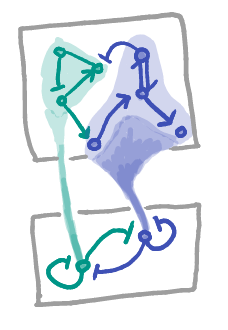
\includegraphics[width=0.9\linewidth]{reduction}
\end{center}
\begin{tcolorbox}[boxrule=2pt,arc=3.4pt,boxsep=2mm]
\begin{center}\color{DarkRed}
\textbf{Using measures of relative complexity between two given networks,
can we construct evolutionary trees and understand how primitive switches
and clocks evolved?}
\end{center}
\end{tcolorbox}
\vfill\null
\columnbreak
\section{Patterns in dynamic populations}
Ever since Turing formulated the differential diffusion condition \cite{}
for pattern formation, whether a biological pattern is truly driven by a
diffusion instability or not has been a matter of debate and speculation.
\\\\
It is conceivable that the differential diffusion condition is satisfied
by the time-scale separation between cytosolic, membrane and inter-cellular
reactions.
\\\\
Finite element reaction-diffusion simulations can take these effects into
account explicity at an enourmous computational cost, which leads researches to
resort to more abstract Kuramoto-type models.
\\
\begin{tcolorbox}[boxrule=2pt,arc=3.4pt,boxsep=2mm]
\begin{center}\color{DarkRed}
\textbf{Can we construct a computationally tractable reaction-diffusion model
that takes cell division and death into account?}
\end{center}
\end{tcolorbox}
\begin{center}
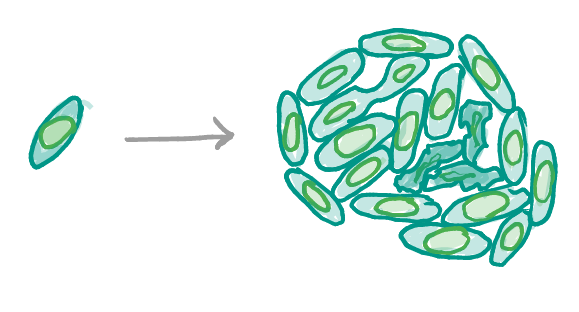
\includegraphics[width=0.9\linewidth]{population}
\end{center}
\vfill\null
\columnbreak
\section{Geometrisation approach}

% %----------------------------------------------------------------------------------------
% %	CONCLUSIONS
% %----------------------------------------------------------------------------------------
%
% \color{SaddleBrown} % SaddleBrown color for the conclusions to make them stand out
%
% \section*{Conclusions}
% Despite being a petroleum- and gas-rich country, Algeria is making efforts to exploit its renewable energies. The Algerian government has adopted new renewable energy laws and financial support for the investors to facilitate the exploitation of the renewable energies for electricity production and direct utilizations. Algeria has relatively abundant geothermal resources especially in the northeastern parts but not totally used.
% \color{Black} % Set the color back to DarkSlateGray for the rest of the content
%
% %----------------------------------------------------------------------------------------
% %	FORTHCOMING RESEARCH
% %----------------------------------------------------------------------------------------
%
% \section*{Forthcoming Research}
%
% Simulation of thermodynamic properties of the thermal fluid and power output with longevity using geological, hydrogeological, and geothermal data from NE-Algerian geothermal reservoirs.
%
%  %----------------------------------------------------------------------------------------
% %	REFERENCES
% %----------------------------------------------------------------------------------------
%
\bibliographystyle{plain} % Plain referencing style
\bibliography{mendeley_v2} % Use the example bibliography file sample.bib

%----------------------------------------------------------------------------------------

\end{multicols}
\end{document}
